%% ----------------------------------------------------------------
%% MAIN FILE 
%% ---------------------------------------------------------------- 

% Set up the document
\documentclass[a4paper, 12pt, oneside]{Thesis}  % Use the "Thesis" style
\graphicspath{images/}                          % Location of the graphics files 

% Table configuration packages
\usepackage{array,graphicx}
\usepackage{booktabs}
\usepackage{pifont}
\usepackage{libertine}
\usepackage{tabu}
\usepackage{longtable}
\usepackage{xcolor}
\usepackage{tcolorbox}
\usepackage{textcomp}
\usepackage{multicol}
%\usepackage{amsthm}

\makeatother

% Include any extra LaTeX packages required
\usepackage[square, numbers, comma, sort&compress]{natbib}          % natbib for the bibliography
\usepackage{verbatim}                                               % Needed to make LaTeX comments
\usepackage{float}                                                  % To keep figures in place
\hypersetup{urlcolor=black, colorlinks=false, pdfborder = {0 0 0}}  % Colours hyperlinks in blue

% Define enumerated description lists
\usepackage{enumitem}
\newcounter{descriptcount}
\newcounter{descriptcount2}
\newlist{enumdescript}{description}{2}
\setlist[enumdescript,1]{%
  before={\setcounter{descriptcount}{0}%
          \renewcommand*\thedescriptcount{\arabic{descriptcount}.}}
  ,font=\bfseries\stepcounter{descriptcount}\thedescriptcount~
}
\setlist[enumdescript,2]{%
  before={\setcounter{descriptcount2}{0}%
          \renewcommand*\thedescriptcount{\roman{descriptcount2}.}}
  ,font=\bfseries\stepcounter{descriptcount2}\thedescriptcount~
}
 
% Theorem, propositions and definitions enviroment
% https://www.overleaf.com/learn/latex/theorems_and_proofs

%\newtheorem{theorem}{Theorem}
%\newtheorem{corollary}{Corollary} %[section]
%\newtheorem{lemma}{Lemma}
%\newtheorem{definition}{Definition}
%\newtheorem{proposition}{Proposition}

% Theorem enviroment example
%\begin{theorem}
%Let $f$ be a function whose derivative exists in every point, then $f$ is 
%a continuous function.
%\end{theorem}
%
%\begin{theorem}[Pythagorean theorem]
%\label{pythagorean}
%This is a theorema about right triangles and can be summarised in the %next 
%equation 
%\[ x^2 + y^2 = z^2 \]
%\end{theorem}

 
%% ----------------------------------------------------------------
%% DOCUMENT START
%% ---------------------------------------------------------------- 
\begin{document}

% Configuration and parameters given in  Thesis.cls file
\frontmatter                % Begin the book's numbering; frontpage
%\pagenumbering{arabic}     % In case we don't want roman numbers enumeration at first

%% ----------------------------------------------------------------

\setstretch{1.3}  % Better to have smaller font and larger line spacing than the other way round

% Define the page headers using the FancyHdr package and set up for one-sided printing
\fancyhead{}      % Clears all page headers and footers
\rhead{\thepage}  % Sets the right side header to show the page number
\lhead{}          % Clears the left side page header

\pagestyle{fancy}  % Finally, use the "fancy" page style to implement the FancyHdr headers

%% ----------------------------------------------------------------
%% TITLE PAGE
%% ---------------------------------------------------------------- 

% Structure: http://www.cyta.com.ar/ta0206/v2n6a3/v2n6a3.htm

\title {Convolutional neural networks for multiple sclerosis lesion detection}

\authors  {\texorpdfstring
            {\href{mailto:francisco.blazquezmartinez@epfl.ch}{Francisco Javier Blázquez Martínez}}
            {Francisco Javier Blázquez Martínez}
            }
\addresses  {\groupname\\\deptname\\\univname}  
\date       {\today}
\subject    {}
\keywords   {}

\maketitle



%% ----------------------------------------------------------------
%% DECLARATION OF AUTHORSHIP
%% ---------------------------------------------------------------- 

\begin{comment}
\Declaration{

\addtocontents{toc}{\vspace{1em}}  % Add a gap in the Contents, for aesthetics

I, Francisco Javier Blázquez Martínez, declare that this thesis titled ``Graver basis'' and the work presented in it are my own. I confirm that:

\begin{itemize} 
\item[\tiny{$\blacksquare$}] This work was done wholly or mainly while in candidature for a research degree at this University.
 
\item[\tiny{$\blacksquare$}] Where any part of this thesis has previously been submitted for a degree or any other qualification at this University or any other institution, this has been clearly stated.
 
\item[\tiny{$\blacksquare$}] Where I have consulted the published work of others, this is always clearly attributed.
 
\item[\tiny{$\blacksquare$}] Where I have quoted from the work of others, the source is always given. With the exception of such quotations, this thesis is entirely my own work.
 
\item[\tiny{$\blacksquare$}] I have acknowledged all main sources of help.
 
\item[\tiny{$\blacksquare$}] Where the thesis is based on work done by myself jointly with others, I have made clear exactly what was done by others and what I have contributed myself.
\\
\end{itemize}
 
 
Signed:\\
\rule[1em]{25em}{0.5pt}  % This prints a line for the signature
 
Date:\\
\rule[1em]{25em}{0.5pt}  % This prints a line to write the date
}
\clearpage  % Declaration ended, now start a new page
\end{comment}

%% ----------------------------------------------------------------
%% ABSTRACT PAGE
%% ---------------------------------------------------------------- 

% TODO: modify the abstract style in thesis.cls file!
\addtotoc{Abstract}
\abstract{



}

\clearpage  % Abstract ended, start a new page

%% ----------------------------------------------------------------
%% ACKNOWLEDGEMENTS
%% ---------------------------------------------------------------- 

\setstretch{1.3}  % Reset the line-spacing to 1.3 for body text (if it has changed)

% The Acknowledgements page, for thanking everyone
\acknowledgements{
\addtocontents{toc}{\vspace{1em}} 

% TODO:
% David Atienza - Por estar yo en la EPFL y poder hacer este proyecto
% Katzalin Olcoz - Por estar en la EPFL y por mi formación en la UCM
% Marina Zapater - Por proponerme y orientar el proyecto
% Arman Iranfar, Tomás Teijeiro, por supervisarme

% Familia, amigos, Ana?

%In the last years, with the increase in biomedical data and the advances in the Artificial Intelligence techniques to exploit these... 


}
\clearpage  % End of the Acknowledgements

\pagestyle{fancy}  %The page style headers have been "empty" all this time, now use the "fancy"

%% ----------------------------------------------------------------
%% DEDICATION
%% ---------------------------------------------------------------- 
% Insert empty page / blank page
%\thispagestyle{empty}
%\null
%\newpage

\pagestyle{empty}  % Page style needs to be empty for this page
\dedicatory{
To my father,\\ for all the things that can only be learnt by example. \\
}



%% ----------------------------------------------------------------
%% INDEX
%% ---------------------------------------------------------------- 

% TODO: I don't like subsections in the index!!

\lhead{\emph{Contents}}  % Set the left side page header to "Contents"
\tableofcontents  % Write out the Table of Contents

%% ----------------------------------------------------------------
%% LIST OF FIGURES
%% ---------------------------------------------------------------- 
\begin{comment}
\lhead{\emph{List of Figures}}  % Set the left side page header to "List if Figures"
\listoffigures  % Write out the List of Figures
\end{comment}

%% ----------------------------------------------------------------
%% LIST OF TABLES
%% ---------------------------------------------------------------- 
\begin{comment}
\lhead{\emph{List of Tables}}  % Set the left side page header to "List of Tables"
\listoftables  % Write out the List of Tables
\end{comment}

%% ----------------------------------------------------------------
%% ABBREVIATIONS
%% ---------------------------------------------------------------- 
\begin{comment}
\setstretch{1.5}  % Set the line spacing to 1.5, this makes the following tables easier to read
\clearpage  % Start a new page
\lhead{\emph{Abbreviations}}  % Set the left side page header to "Abbreviations"
\listofsymbols{ll}  % Include a list of Abbreviations (a table of two columns)
{
\textbf{Acronym} & \textbf{W}hat (it) \textbf{S}tands \textbf{F}or \\
% Abbreviations go here
}

\lhead{}

\setstretch{1.3}  % Return the line spacing back to 1.3

\end{comment}

%% ----------------------------------------------------------------
%% INCLUDE ALL SECTIONS
%% ---------------------------------------------------------------- 
\mainmatter	       % Begin normal, numeric (1,2,3...) page numbering
\pagestyle{fancy}  % Return the page headers back to the "fancy" style

% Include the chapters of the thesis, as separate files
% Just uncomment the lines as you write the chapters

\chapter{Introduction} 
\label{1.Introduction}
\lhead{\emph{Introduction}}


In the last years, with the increase of the available biomedical data and the computation power in GPUs together with the appearance of new Artificial Intelligence (AI) models and techniques, it has existed and exists a growing interest and research effort on applying Artificial Intelligence to several biomedical tasks. In many of these tasks, most of them currently performed manually by doctors or medicine professionals, there have appeared automatic tools based on Artificial Intelligence models which show a performance close to the accuracy of a doctor. In other words, the application of Artificial Intelligence to medicine has proved to be useful and is definitely part of the future of the discipline. It will help by saving doctor's time, increasing the efficiency and the scope of the medicine professionals, helping them to provide more accurate diagnoses or even creating diagnoses by themselves and ultimately contributing to save lives.

Aware of this, the European Comission starts in 2019 the DeepHealth project. This aims to offer a unified framework completely adapted to exploit underlying heterogeneous High-Performance Computing (HPC) and Big Data architectures, framework to be assembled with state-of-the-art techniques in Deep Learning (DL) and Computer Vision. In particular,the project combines High-Performance Computing infrastructures with Deep Learning (DL) and Artificial Intelligence techniques to support biomedical applications that require the analysis of large and complex biomedical datasets and thus, new and more efficient ways of diagnosis, monitoring and treatment of diseases. The framework consist on two general purpopse libraries which are currently being developed, EDDL for Deep Learning computing infrastructure and ECVL for computer vision tools. 

The goal of this project is to create state-of-the art Deep Learning models to detect of Multiple Sclerosis (MS) lesions in Magnetic Resonance Images (MRI) using EDDL library, analyzing its performance and comparing it with other commonly used libraries.



\section{Multiple Sclerosis}

Multiple sclerosis is the most common immune-mediated disorder affecting the central nervous system.
% TODO: Continue introduction about Multiple Sclerosis



\newpage
\section{Multiple Sclerosis lesion segmentation}

Multiple Sclerosis lesion segmentation consists on identifying in an MRI the damaged parts of the brain. This task plays a role in every stage of the disease, it has a huge importance in the patients for an early diagnose, for following the evolution of the disease and for measuring the effects of the treatment. However, this task has to be done manually by experts and involves analyzing a huge amount of data so it's highly time-consuming and prone to errors. Considering also the how relatively common this disease is, it's clear the importance of trying to optimize it. In fact, MS lesion segmentation was established as one of the main use cases for the development of the DeepHealth project. 

MS lesion segmentation is a difficult task \textit{per se}, but even more given the difficulty and cost of obtaining and labeling the data. This makes almost impossible for anybody without the needed resources to access to a dataset and, in the best case, to have only a few samples, what makes almost any Machine Learning approach to be unfeasible. However, in recent years, within MICCAI2008 and MICCAI2016 challenges, there have been a big research effort which has led to the emergence of various different approaches and solutions. These include the usage of classical image segmentation networks\cite{MICCAI_MSSEG:2016}, Random Forests \cite{MICCAI_MSSEG:2016}, Hybrid Artificial Neural Networks \cite{MICCAI_MSSEG:2016}, Automated Multimodal Graph Cut \cite{MICCAI_MSSEG:2016}, unsupervised approaches using Rules and Level Sets \cite{MICCAI_MSSEG:2016}... 

In this project we'll focus our attention on the state-of-the-art approaches using 2-D and 3-D Convolutional Neural Networks (CNN). 

We first analyze the application of 2-D CNN, starting with the U-Net as the standard for biomedical image segmentation, building, training, evaluating and profiling the model. Then we try a newer approach, the Double U-Net, which has proved to improve U-Net in some datasets, comparing both the performance of EDDL library with respect to a keras-tensorflow implementation and the models between themselves.

By last, we analyze the application of a cascade 3-D CNN. Evaluating and profiling the model and comparing it to an equivalent implementation with keras-tensorflow.

% TODO: Reference to the different approaches for MS LS
% TODO: Importance of the task (time consuming, errors...)
% TODO: Importance of the task (evolution, life of patient)
% TODO: MICCAI 2016 and MICCAI 2008 solutions proposed
% TODO: One of the main use cases of the DeepHealth project.







% TODO: Links to EDDL and ECVL
% TODO: Links to DeepHealth project webpage
% TODO: EDDL versions? % Introduction

\chapter{Data} 
\label{2.Data}
\lhead{\emph{Data}}

% https://www.datacamp.com/community/tutorials/matplotlib-3d-volumetric-data


% Todo empieza con MICCAI2008
% Explota con MICCAI2016

% TODO: Improve
The two main datasets for MS lesion segmentation are those for MICCAI 2008 and MICCAI 2016 challenges. In this project we'll work over MICCAI 2016 dataset.

\section{MICCAI 2016 dataset}

% TODO: Modalities/Channels!!
MICCAI 2016 dataset consists on 15 MRIs together with a lession mask generated by consensus among various doctors. These are generated with three different scanners, each one with a certain data shape. We verified that all the MRIs are present with the same orientation, what will be meaningfull when slicing the 3-D MRIs for the 2-D models. The dataset contains also preprocessed data in which the skull has been removed from the MRIs, for simplicity, we'll be using these for all the models.

We split randomly the data in a train and a validation set with size 12 and 3 MRIs respectively. We don't keep a test set because given the fact that the size of this would be reduced to only one or two MRIs at most and the inhomogeneity in the different lesions shape, size, quantity and distribution, the evaluation over the test set would lead to a unreliable measurement. This is something certain after seeing the big differences in the metrics over different validation MRIs. Therefore we encourage to everyone who wants to use this models in practice to previously evaluate them over his own data.

We present in the next page some slices of MRIs used as benchmarks for error detection and visual analysis of the models from both the train and validation datasets.

\newpage
Becnhmark training images:
\begin{figure*}[!htb]
    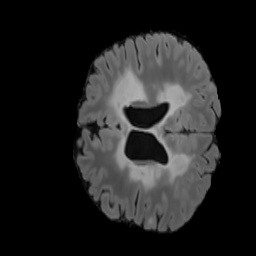
\includegraphics[width=.32\textwidth]{images/tr_images/tr175_input.jpg}\hfill
    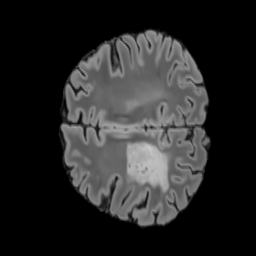
\includegraphics[width=.32\textwidth]{images/tr_images/tr943_input.jpg}\hfill
    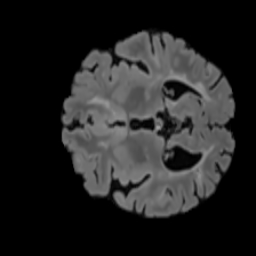
\includegraphics[width=.32\textwidth]{images/tr_images/tr1426_input.jpg}
    %\caption{Image A.}
    %\caption{Image B.}
    %\caption{Image C.}
    \subfigure[tr175]{
\includegraphics[width=.32\textwidth]{images/tr_images/tr175_mask.jpg}\label{fig:tr175}}\hfill
    \subfigure[tr943]{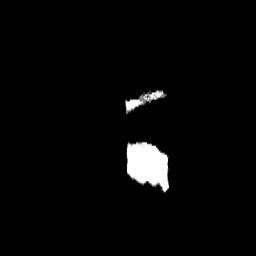
\includegraphics[width=.32\textwidth]{images/tr_images/tr943_mask.jpg}\label{fig:tr943}}\hfill
    \subfigure[tr1426]{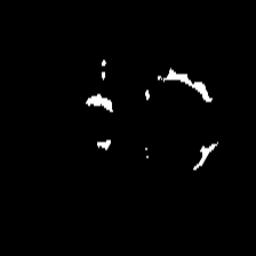
\includegraphics[width=.32\textwidth]{images/tr_images/tr1426_mask.jpg}\label{fig:tr1426}}
    %\caption{Image A.}
    %\caption{Image B.}
    %\caption{Image C.}
\end{figure*}

Benchmark validation images: 
\begin{figure*}[!htb]
    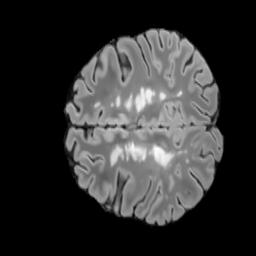
\includegraphics[width=.32\textwidth]{images/ts_images/ts175_input.jpg}\hfill
    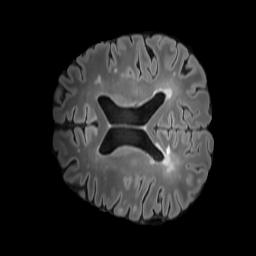
\includegraphics[width=.32\textwidth]{images/ts_images/ts431_input.jpg}\hfill
    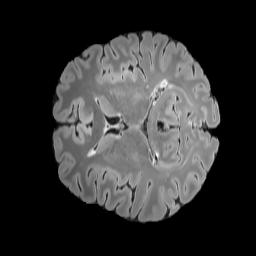
\includegraphics[width=.32\textwidth]{images/ts_images/ts687_input.jpg}
    %\caption{Image A.}
    %\caption{Image B.}
    %\caption{Image C.}
    \subfigure[ts175]{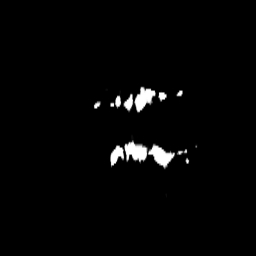
\includegraphics[width=.32\textwidth]{images/ts_images/ts175_mask.jpg}\label{fig:ts175}}\hfill
    \subfigure[ts431]{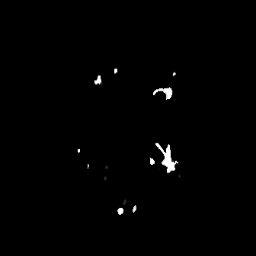
\includegraphics[width=.32\textwidth]{images/ts_images/ts431_mask.jpg}\label{fig:ts431}}\hfill
    \subfigure[ts687]{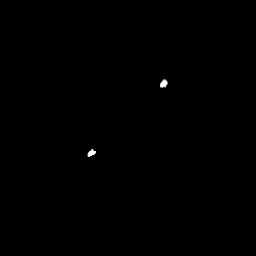
\includegraphics[width=.32\textwidth]{images/ts_images/ts687_mask.jpg}\label{fig:ts687}}
    %\caption{Image A.}
    %\caption{Image B.}
    %\caption{Image C.}
\end{figure*}

\newpage
\section{Evaluation metrics}

%%%%%%%%%%%%%%%%%% Listing configuration %%%%%%%%%%%%%%%%%
\definecolor{gray97}{gray}{.97}
\definecolor{gray75}{gray}{.75}
\definecolor{gray45}{gray}{.45}

\lstset{ frame=Ltb,
framerule=0pt,
aboveskip=0.5cm,
framextopmargin=3pt,
framexbottommargin=3pt,
framexleftmargin=0.4cm,
framesep=0pt,
rulesep=.4pt,
backgroundcolor=\color{gray97},
rulesepcolor=\color{black},
%
stringstyle=\ttfamily,
showstringspaces = false,
basicstyle=\fontsize{9.5}{10}\selectfont\ttfamily,
commentstyle=\color{gray45},
keywordstyle=\bfseries,
%
numbers=left,
numbersep=15pt,
numberstyle=\tiny,
numberfirstline = false,
breaklines=true,
}

% minimizar fragmentado de listados
\lstnewenvironment{listing}[1][]
{\lstset{#1}\pagebreak[0]}{\pagebreak[0]}

\lstdefinestyle{consola}
{basicstyle=\scriptsize\bf\ttfamily,
backgroundcolor=\color{gray75},
}

\lstdefinestyle{C}
{language=Python,
}
%%%%%%%%%%%%%%%%%%%%%%%%%%%%%%%%%%%%%%%%%%%%%%%%%%%%%%%%%%

During the training processes we have used \textit{binary cross entropy} as loss function. For evaluation we have used the \textit{Dice score}, a classical metric for image segmentation, much more representative than others used in classification tasks as \textit{Mean Squared Error} or \textit{Binary accuracy}. \textit{Dice score} is implemented in several similar but not fully equivalent ways and it's not a built-in metric in keras-tensorflow so we had to create our custom implementations for both the tensorflow and PyEDDL models. This way we also ensure they are strictly equivalent.

\begin{equation*}
Dice(Pred, Mask) = 2*\frac{|Pred \cap Mask |}{|Pred| + |Mask|} 
\end{equation*}
\vspace{10pt}

\begin{lstlisting}[language=Python, caption=Keras backend Dice implementation]
import keras.backend as K

def dice(y_true, y_pred, smooth=1):
    intersection = K.sum(y_true * y_pred, axis=[1,2,3])
    union = K.sum(y_true, axis=[1,2,3]) + K.sum(y_pred, axis=[1,2,3])
    dice = K.mean((2. * intersection + smooth)/(union + smooth), axis=0)
    return dice
\end{lstlisting}

\begin{lstlisting}[language=Python, caption=PyEDDL Dice implementation]
from pyeddl._core  import Metric

class Dice(Metric):
    def __init__(self, threshold=0.5):
        Metric.__init__(self, "py_dice")
        self.threshold = threshold

    def value(self, msk, out, smooth=1):   
        out_np = out.getdata() >= self.threshold
        msk_np = msk.getdata().astype(np.bool)
        intersection = np.logical_and(msk_np, out_np)
        
        dice = 0
        for i in range(msk_np.shape[0]):
            union_i = np.sum(msk_np[i]) + np.sum(out_np[i])
            dice += (2*np.sum(intersection[i])+smooth) / (union_i+smooth)

        return dice

\end{lstlisting} % Dataset explanation

\chapter{2-D Convolutional Nerual Networks}
\label{3.2D_CNN}

\chapter{3-D Convolutional Nerual Networks}
\label{4.3D_CNN}
\lhead{\emph{3-D Convolutional Neural Networks}}

\section{Data preprocessing}

\section{Cascade model}


%% ----------------------------------------------------------------
%% APPENDICES
%% ---------------------------------------------------------------- 
%\addtocontents{toc}{\vspace{2em}} % Add a gap in the Contents, for aesthetics

\appendix % Cue to tell LaTeX that the following 'chapters' are Appendices

% Appendix A
%\input{src/8.ApendixA} 

% Appendix B
\chapter{Apendix title} 
\label{ApendixA}
 

% Example appendices

\addtocontents{toc}{\vspace{2em}}  % Add a gap in the Contents, for aesthetics
\backmatter % End the book's numbering; backpage

%% ----------------------------------------------------------------
%% BIBLIOGRAPHY
%% ---------------------------------------------------------------- 

% References:
% https://www.latex-tutorial.com/tutorials/bibtex/
% https://www.overleaf.com/learn/latex/Bibliography_management_in_LaTeX

\label{Bibliography}
\lhead{\emph{Bibliography}}  % Change the left side page header to "Bibliography"
%\bibliographystyle{plain}
\bibliographystyle{unsrtnat}  % Use the "unsrtnat" BibTeX style for formatting the Bibliography

\nocite{*}
\bibliography{Bibliography}  % The references (bibliography) information are stored in the file named "Bibliography.bib"

\end{document}  % The End
%% ----------------------------------------------------------------